% INF-221 Tarea 1 2026-2 | Tomás San Martín | Rol 202473565-9
\subsection{Ordenamiento}
\begin{figure}[ht]\centering
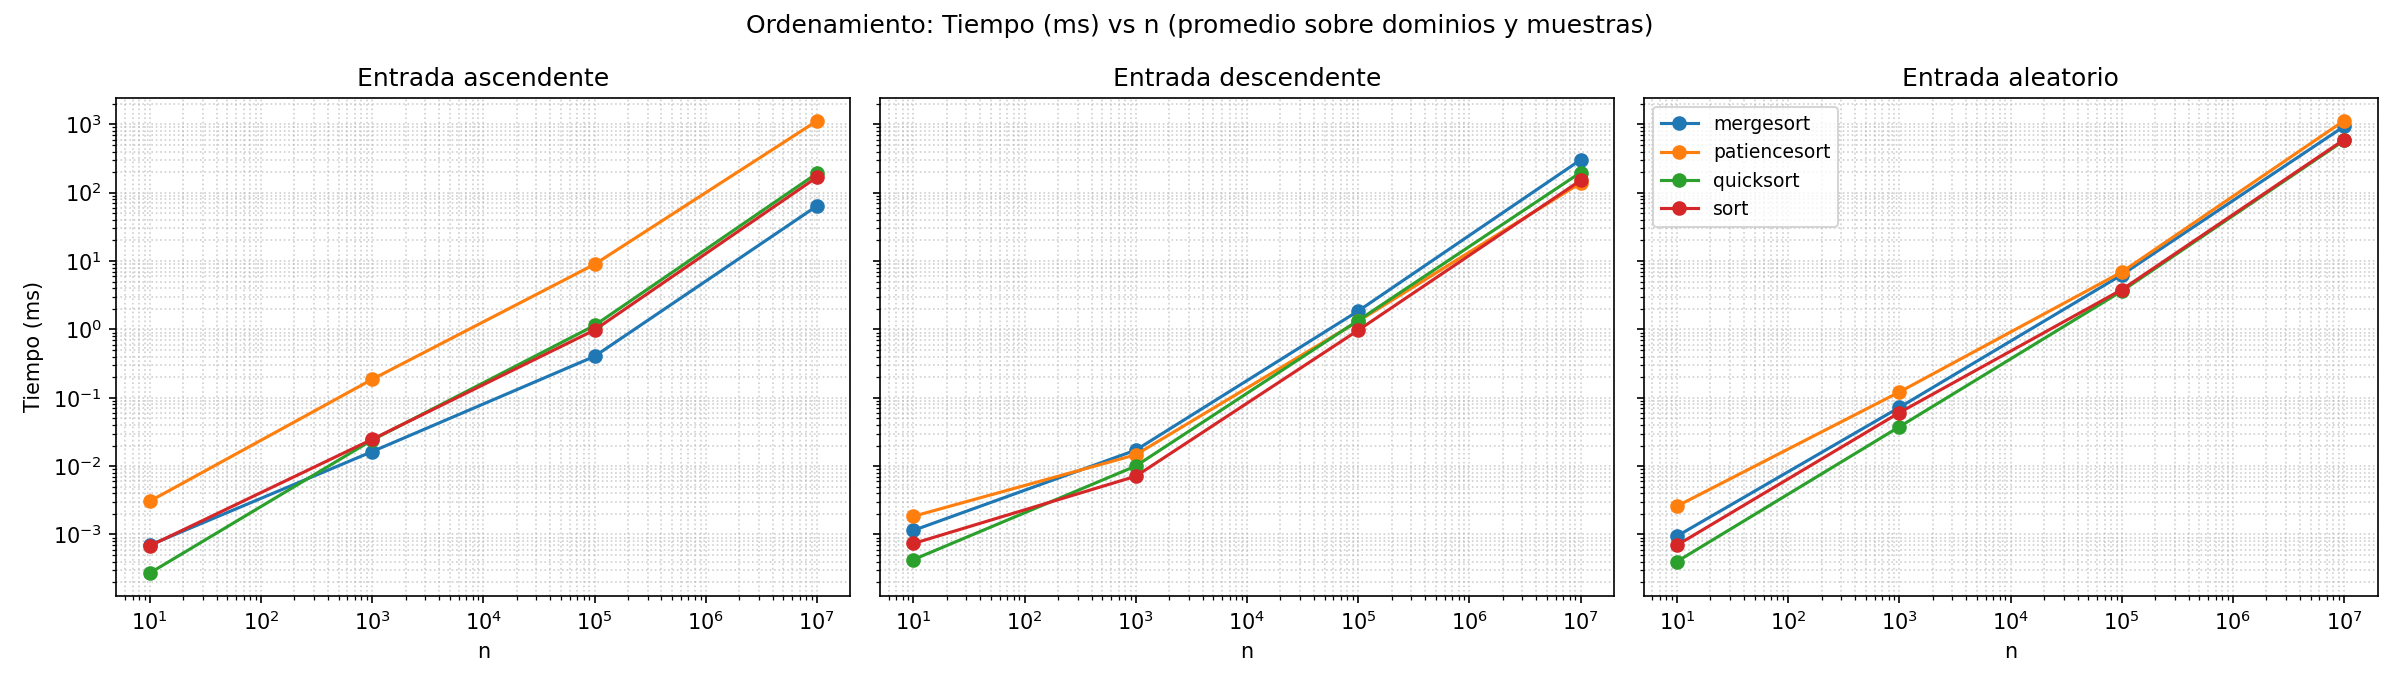
\includegraphics[width=\textwidth]{figs/tiempos_sorting.png}
\caption{Tiempo de ordenamiento vs $n$ (escala log--log), promedio sobre dominios y muestras.}
\end{figure}
\begin{figure}[ht]\centering
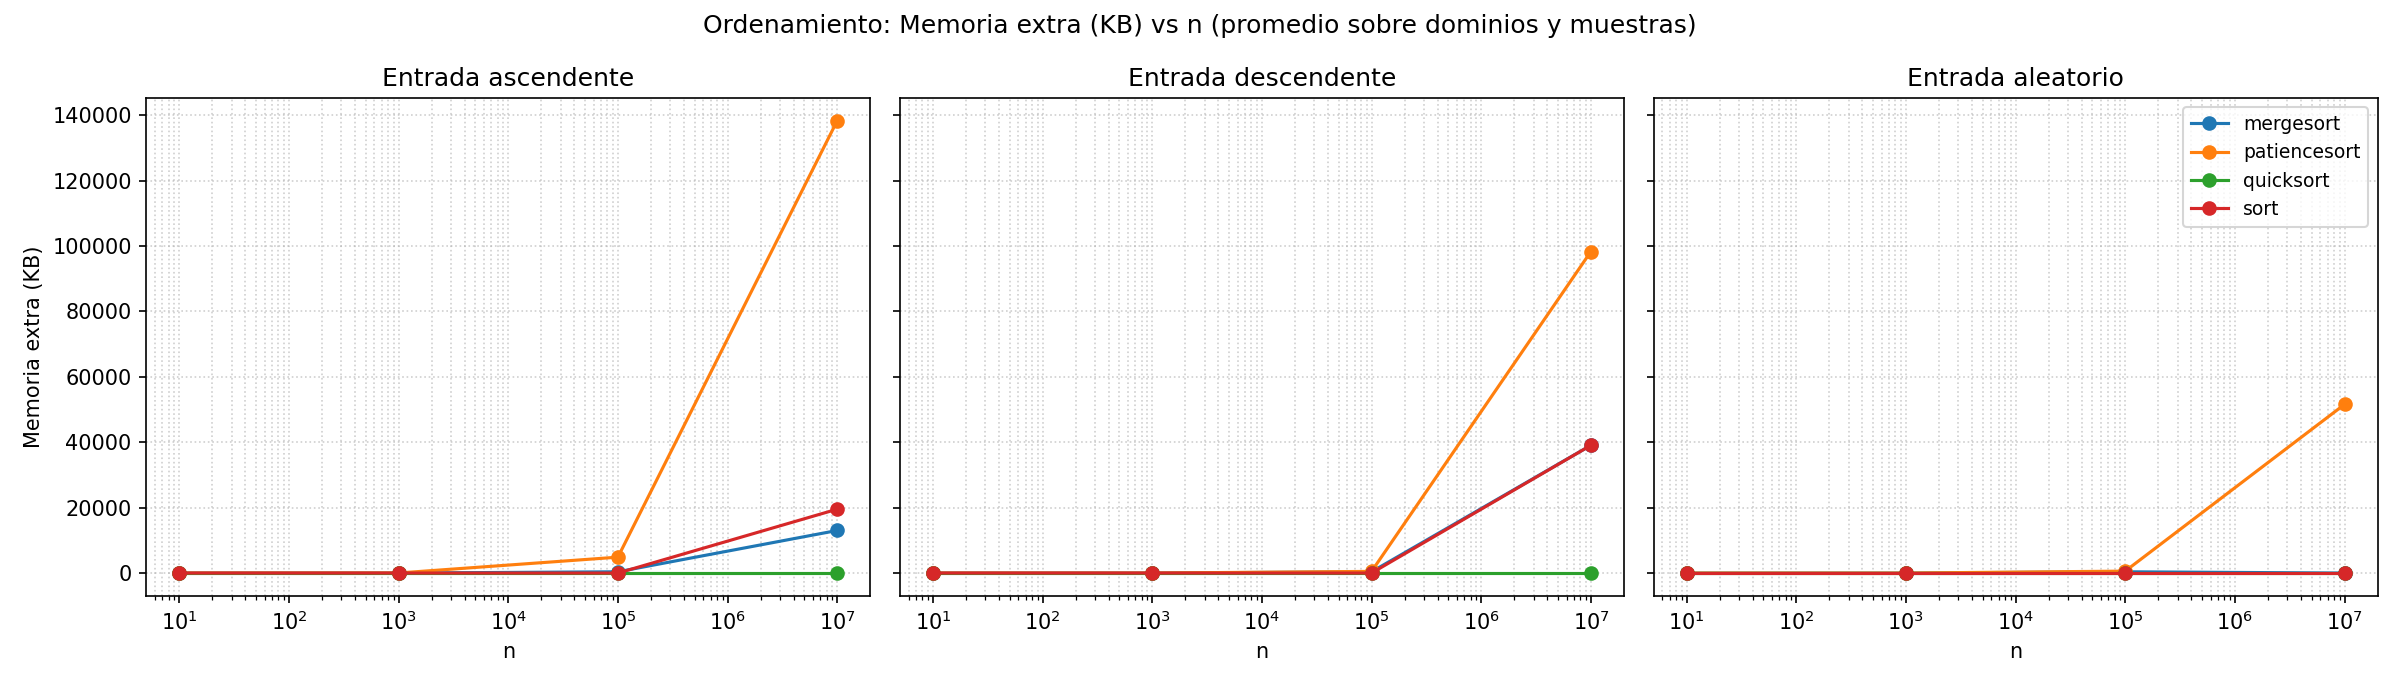
\includegraphics[width=\textwidth]{figs/memoria_sorting.png}
\caption{Memoria extra de ordenamiento vs $n$.}
\end{figure}
\begin{table}[ht]\centering
\caption{Tiempo (ms), entrada aleatoria, dominio D7, muestra a.}
\begin{tabular}{l|rrrr}
\hline
$n$ & merge & quick & patience & std::sort \\ \hline
$10^5$  & 7.98 & 5.17 & 10.26 & 5.42 \\
$10^7$  & 1247.82 & 867.64 & 1870.45 & 862.97 \\ \hline
\end{tabular}
\end{table}
En escala log--log las curvas presentan pendiente cercana a 1, coherente con
$O(n\log n)$. \texttt{std::sort} y quick sort dominan en entrada aleatoria;
merge sort es el más rápido en entrada ascendente gracias a la fusión
condicional, mientras que patience sort se degrada notablemente en ese caso
porque genera aproximadamente $n$ pilas. En memoria, merge y patience crecen
lineales ($O(n)$: buffer y pilas más arreglo de salida), en tanto que quick
sort y \texttt{std::sort} permanecen planos: su espacio extra es pila de
recursión $O(\log n)$, no heap.
\subsection{Multiplicación de matrices}
\begin{figure}[ht]\centering
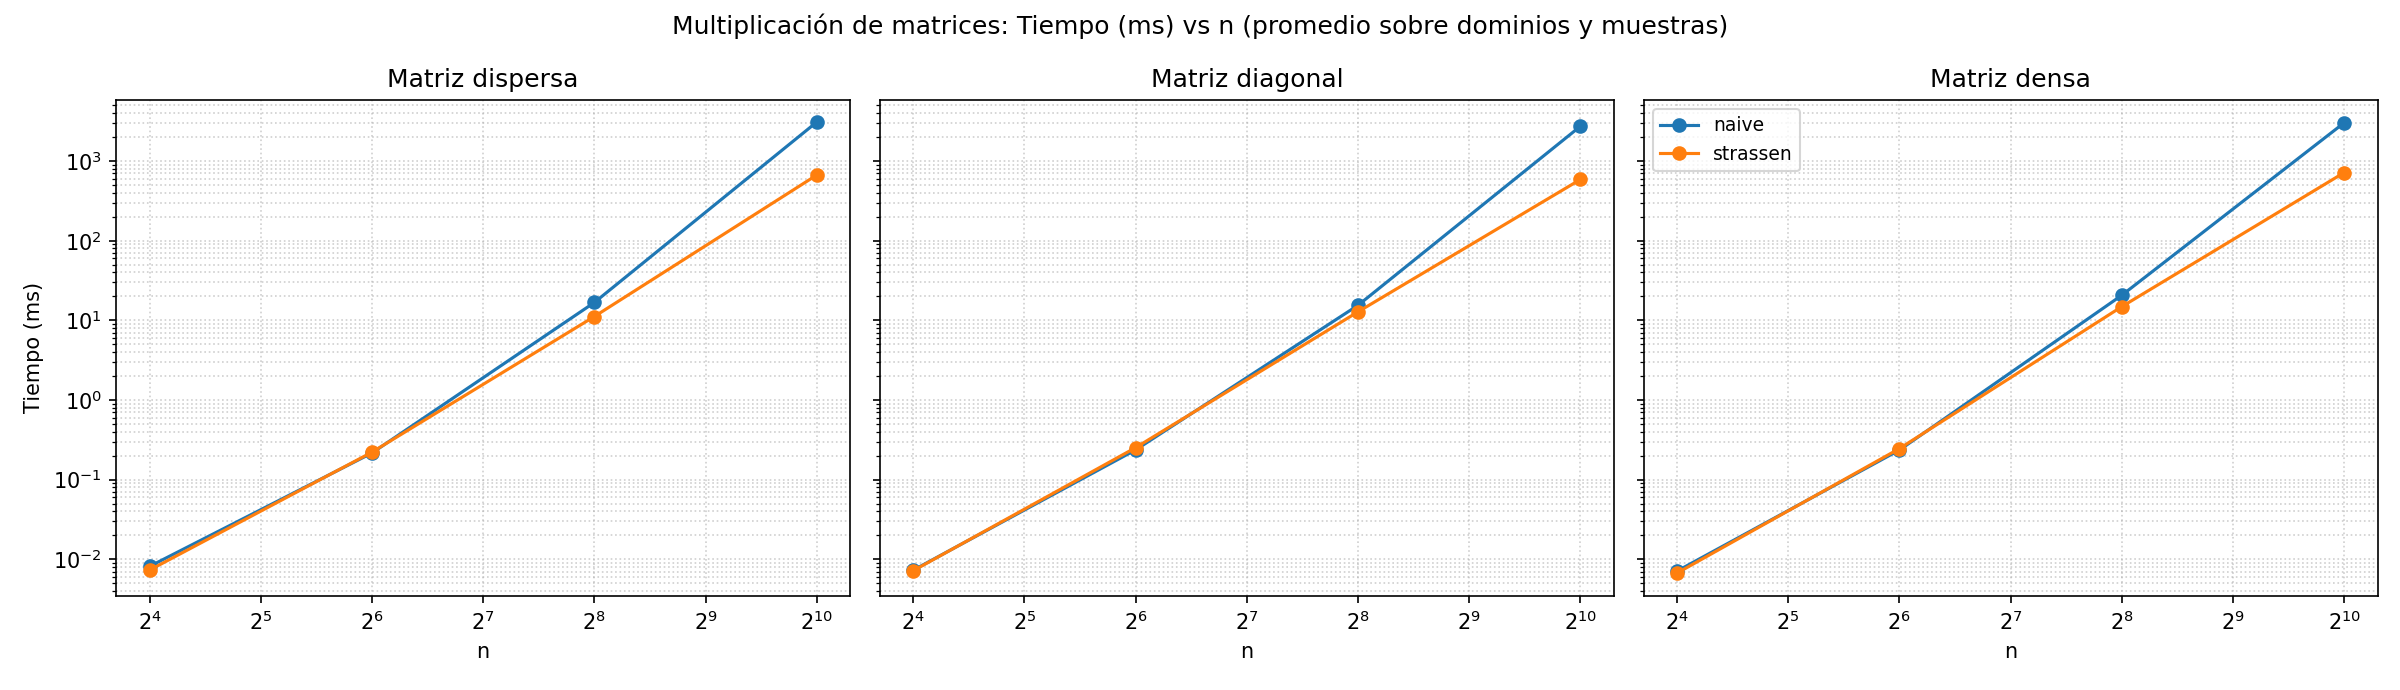
\includegraphics[width=\textwidth]{figs/tiempos_matrices.png}
\caption{Tiempo de multiplicación vs $n$ (log--log).}
\end{figure}
\begin{figure}[ht]\centering
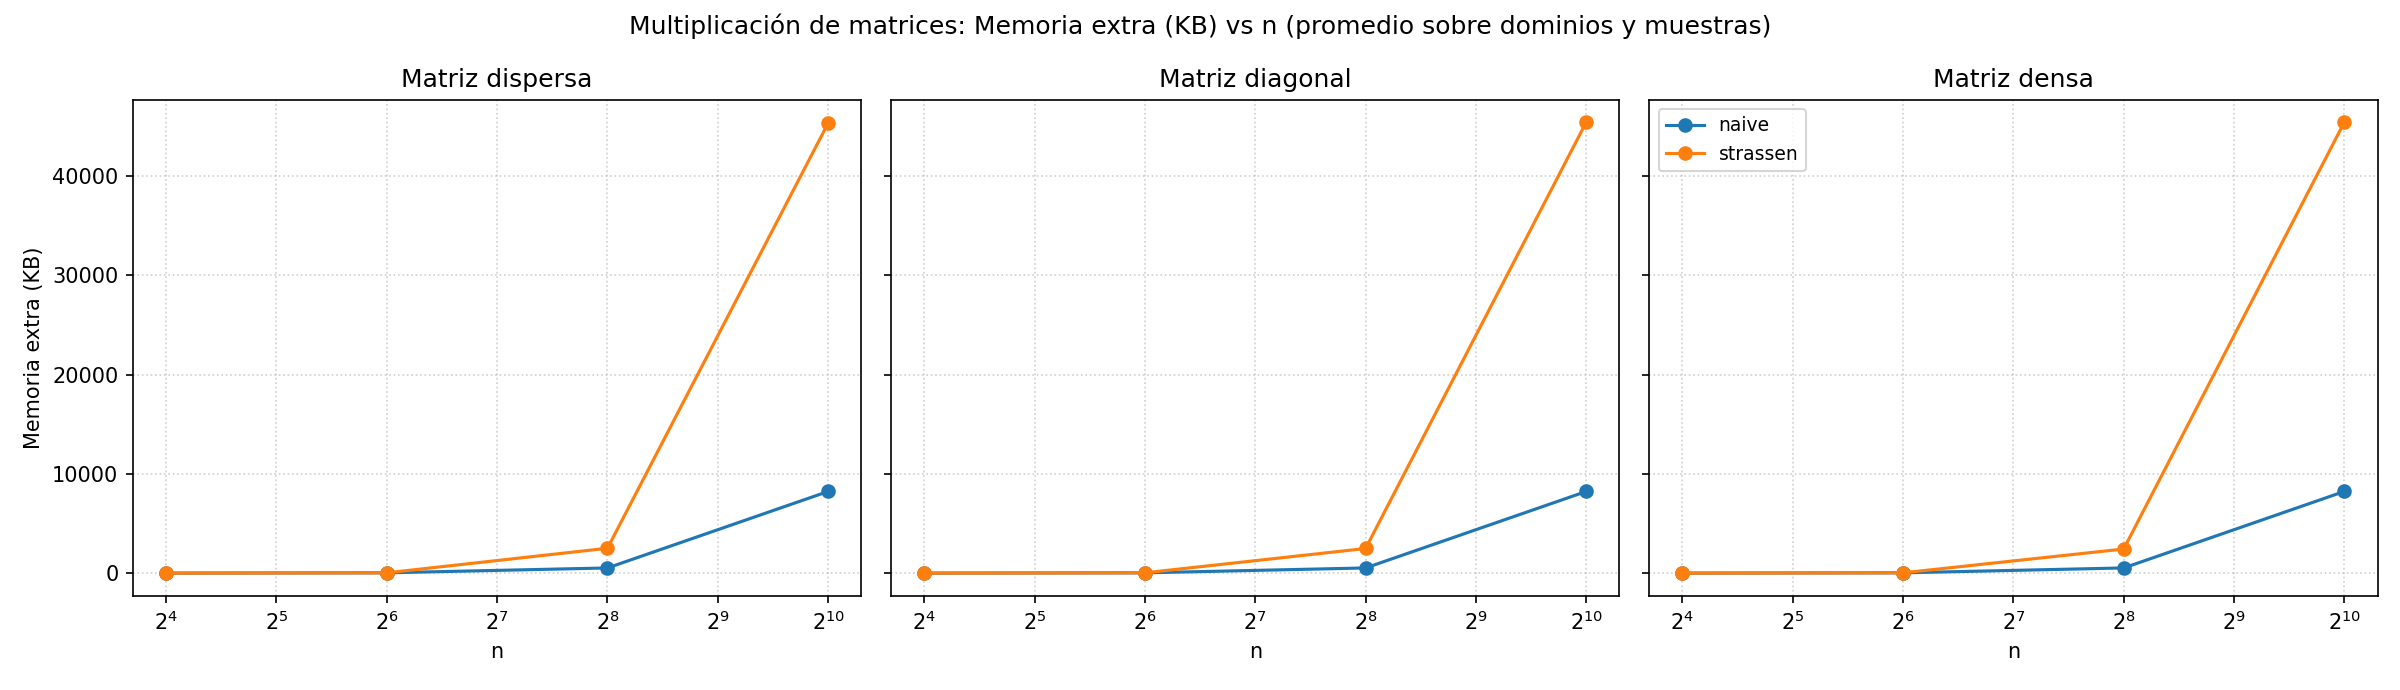
\includegraphics[width=\textwidth]{figs/memoria_matrices.png}
\caption{Memoria extra de multiplicación vs $n$.}
\end{figure}
\begin{table}[ht]\centering
\caption{Tiempo (ms), matriz densa, dominio D10, muestra a.}
\begin{tabular}{l|rr}
\hline
$n$ & naive & strassen \\ \hline
$2^8$   & 16.62 & 13.24 \\
$2^{10}$ & 3296.23 & 712.13 \\ \hline
\end{tabular}
\end{table}
Naive exhibe pendiente $\approx 3$ ($O(n^3)$) y Strassen $\approx 2.81$
($O(n^{\log_2 7})$). El cruce aparece entre $2^8$ y $2^{10}$: la constante
oculta de Strassen (siete productos recursivos más las sumas de matrices) solo
se amortiza en tamaños grandes. En memoria, naive asigna únicamente la matriz
resultado ($\approx 8$\,MB en $n=1024$), mientras Strassen alcanza
$\approx 45$\,MB por los temporales recursivos: el divide-and-conquer compra
tiempo con espacio.